\documentclass[8pt, xcolor={svgnames}, hyperref={colorlinks,linkcolor=black, citecolor=amethyst, urlcolor=amethyst}]{beamer}


\usepackage[labelfont={color=amethyst,bf}]{caption}
\usetheme[progressbar=frametitle]{metropolis}
\usepackage{appendixnumberbeamer}
\usepackage{url}
\usepackage{booktabs}
\usepackage{braket}
\usepackage[scale=2]{ccicons}
\usepackage{amsfonts} 
\usepackage{amssymb}
\usepackage[english]{babel}
\colorlet{col1}{teal}
\colorlet{col2}{yellow}
\colorlet{col3}{green}
\usepackage{fontawesome}
\usepackage{multicol}
\usepackage{bm}
\usepackage{algorithm}
\usepackage{algpseudocode}
\usepackage{enumitem}

\usepackage[]{pseudo}


\usepackage{tikz}
\usetikzlibrary{positioning,arrows,calc,math,angles,quotes}
\usepackage{blochsphere}

\usetikzlibrary{arrows,automata}
\usetikzlibrary{positioning}
\usetikzlibrary{arrows.meta,
                bending,
                intersections,
                quotes,
                shapes.geometric}

\tikzset{
    state/.style={
           rectangle,
           rounded corners,
           draw=black, very thick,
           minimum height=1em,
           inner sep=2pt,
           text centered,
           },
}


\definecolor{myv}{rgb}{0.36, 0.22, 0.33}
\definecolor{gio}{rgb}{0.45, 0.31, 0.59}
\definecolor{light}{rgb}{0.8, 0.8, 1}
\definecolor{warmblack}{rgb}{0.0, 0.26, 0.26}
\definecolor{brown(web)}{rgb}{0.65, 0.16, 0.16}
\definecolor{cadmiumgreen}{rgb}{0.0, 0.42, 0.24}
\definecolor{darkmidnightblue}{rgb}{0.0, 0.2, 0.4}
\definecolor{brightube}{rgb}{0.82, 0.62, 0.91}

\definecolor{codegreen}{rgb}{0,0.6,0}
\definecolor{codegray}{rgb}{0.5,0.5,0.5}
\definecolor{codepurple}{rgb}{0.58,0,0.82}
\definecolor{backcolour}{rgb}{0.95,0.95,0.92}
\definecolor{amethyst}{rgb}{0.6, 0.4, 0.8}

\definecolor{light-gray}{gray}{0.95}
\newcommand{\code}[1]{\colorbox{light-gray}{\texttt{#1}}}

\usepackage{listings}
\lstdefinestyle{mystyle}{
    backgroundcolor=\color{backcolour},   
    commentstyle=\color{codegreen},
    keywordstyle=\color{codepurple},
    numberstyle=\tiny\color{codepurple},
    stringstyle=\color{magenta},
    basicstyle=\scriptsize,
    breakatwhitespace=false,         
    breaklines=true,                 
    captionpos=b,                    
    keepspaces=true,                 
    numbers=left,                    
    numbersep=5pt,                  
    showspaces=false,                
    showstringspaces=false,
    showtabs=false,                  
    tabsize=2
}

\lstset{style=mystyle}
\usepackage[most]{tcolorbox}
\usepackage{xcolor}

%\usepackage[citecolor = green, linkcolor = blue, bookmarks=true, urlcolor=blue,
%colorlinks=true, pagebackref=true]{hyperref}



%\usepackage{xspace}

\title{QTI-TH Forum: introduction to Quantum Machine Learning}
\date{Jen. 26, 2023}
\author[Matteo Robbiati]{Matteo Robbiati}
\titlegraphic{
\begin{tikzpicture}[overlay, remember picture]
\node[at=(current page.south east), anchor=south east] {%

\includegraphics[width=.15\textwidth]{figures/unimi.png} 
\includegraphics[width=.2\textwidth]{figures/infn_logo.png} 
\includegraphics[width=.25\textwidth]{figures/CERN-Logo.png}  
};
\end{tikzpicture}
}


\begin{document}

\maketitle

\section{A snapshot of Machine Learning}


\begin{frame}{Machine Learning}
    \begin{figure}[H]
\centering
  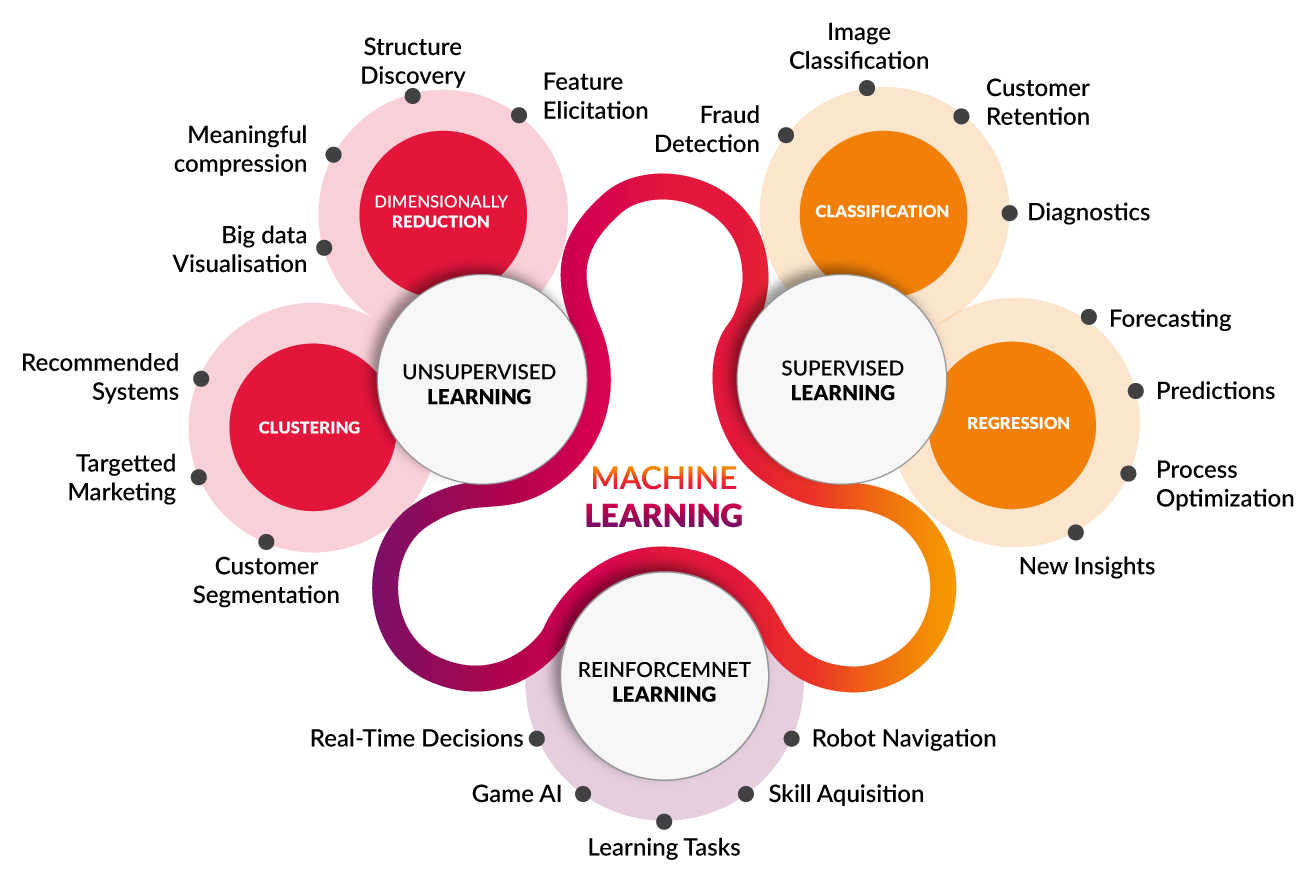
\includegraphics[width=1\linewidth]{figures/ml_types.png}
\end{figure}
\end{frame}

\begin{frame}{A possible definition of ML}
    \large
    
    \begin{tcolorbox}[colback=amethyst!20, title=Machine Learning]
    
    Sub-discipline of both \textbf{artificial intelligence} 
    and \textbf{statistics}, which provides us with a set of tools (algorithms, models) 
    through which \textbf{we can teach a computer} to perform certain tasks, such 
    as pattern recognition, classification, regression, clustering, etc.
    \end{tcolorbox}

\pause

    \vspace{0.5cm}

    \faArrowCircleRight\,\, If we want to implement a machine learning strategy, 
    we need some basic elements:
    \begin{itemize}[noitemsep]
        \item[\faEdit] a model $\mathcal{M}$;
        \item[\faWrench] an optimizer $\mathcal{O}$;
        \item[\faPaypal] a \textbf{loss} (or \textbf{cost}) function $\mathcal{J}$.
        
    \end{itemize}
\end{frame}

\section{ML ingredients}


\begin{frame}{ML - Model $\mathcal{M}$}
\large

\faArrowCircleRight\,\, Let's consider two variables $x$ and $y$ (respectively 
\textbf{input} and \textbf{output} variables), for which we know some theoretical 
relationship $f$ exists.

\pause

\faArrowCircleRight\,\, In supervised ML we have three representation of $f$:

\pause

\begin{itemize}[noitemsep]
    \item[\tiny\faCircle] the true law: $y_{true}=f(x)$;

    \pause
    \item[\tiny\faCircle] our theoretical estimation using a parametric model: 
    $ y_{est} = \mathcal{M}(x | \bm{\theta})$;

    \pause
    \item[\tiny\faCircle] the measured value from a data sample: $y_{meas} = f(x) + \varepsilon$.
\end{itemize}
\pause

\vspace{0.5cm}
\begin{tcolorbox}[colback=amethyst!20, title=Supervised ML goal]
To optimize the parameters of a model\footnote{We can choose the model we prefer.}  
$\mathcal{M}$ so that $y_{est}$ and $y_{meas}$ are as close as possible\footnote{But without falling into over-learning!}.
\end{tcolorbox}

\end{frame}

\begin{frame}{ML - Loss function $\mathcal{J}$}
\large
    \faArrowCircleRight\,\, $\mathcal{J}$ is a function which quantifies the 
    distance between $y_{meas}$ and $y_{est}$:
    $$\mathcal{J} \equiv \mathcal{J}\bigl[y_{meas}, y_{est}\bigr] = \mathcal{J}\bigl[y_{meas}(x), \mathcal{M}(x| \bm{\theta})\bigr].$$

\pause
\faArrowCircleRight\,\, Several $\mathcal{J}$ exist:
\begin{itemize}
    \item[\tiny\faCircle] \textbf{Mean Squared Error}: 
    $$ \mathcal{J}_{mse} \equiv N_{sample}^{-1}\sum_{i=1}^{N_{sample}} \bigl[y_{meas}(x_i) - \mathcal{M}(x_i| \bm{\theta})\bigr]^2;$$
    \item[\tiny\faCircle] \textbf{Accuracy} in a classification problem;
    \item[\tiny\faCircle] \textbf{Categorical cross-Entropy} in multi-class classifications;
    \item[\tiny\faCircle] etc.
\end{itemize}

\pause

\vspace{0.5cm}
\begin{tcolorbox}[colback=amethyst!20, title=Optimization goal]
We search for $\bm{\theta}_{best}$ which minimize $\mathcal{J}$.
\end{tcolorbox}
    
\end{frame}

\begin{frame}{ML - Optimizer $\mathcal{O}$}
\large
\faArrowCircleRight\,\, $\mathcal{O}$ is the object which performs the optimization strategy. Also here different options exist:

\pause
\begin{itemize}
    \item[\faLeaf] \textbf{heuristic algorithms} (annealing, genetic algos, etc.);

    \pause
    \item[\faEdit] \textbf{analytical methods} if the system is solvable;

    \pause
    \item[\faCogs] \textbf{gradient-based} optimizers, performing steps like $\theta_{i} = \theta_{i-1} - \eta \partial_{\theta_i}\mathcal{J}$.
\end{itemize}

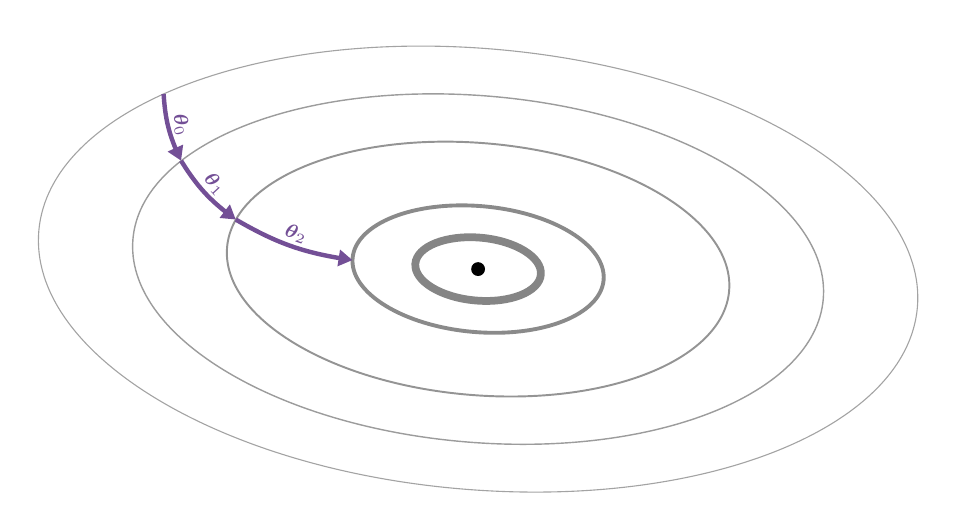
\begin{tikzpicture}[
every edge/.style = {draw, -{Triangle[angle=60:1pt 3,flex]},
bend right=11, gio ,ultra thick},
every edge quotes/.style = {font=\scriptsize, inner sep=1pt, auto, sloped}
                            ]
\fill (0,0) circle[radius=2.5pt];
\path[name path=C] foreach \i in {4, 8, 16, 22, 28}
        {(0,0) circle[draw=red!\i, x radius=2*\i mm, y radius=\i mm, rotate=-5]};
\foreach \i in  {4, 8, 16, 22, 28}
    \draw[line width=11.2/\i, draw=white!\i!gray]
        (0,0) circle[x radius=2*\i mm, y radius=\i mm, rotate=-5];
\path[name path=V] (-4,2.4) .. controls + (0,-2) and + (-2,0) .. (0,0);
%
\draw [name intersections={of=C and V, sort by=C, name=A}]
        (A-5) edge ["$\bm{\theta}_0$"] (A-4)
        (A-4) edge ["$\bm{\theta}_1$"] (A-3)
        (A-3) edge ["$\bm{\theta}_2$"] (A-2);
    \end{tikzpicture}

    
\end{frame}

\begin{frame}{Summing up}
    \begin{figure}[H]
\centering
  \includegraphics[width=1\linewidth]{figures/ml_summary.png}
\end{figure}
\end{frame}

\section{Quantum Machine Learning}

% SLIDE UNO QML
\begin{frame}{Quantum Machine Learning - doing ML using QC}

\vspace{1.5cm}


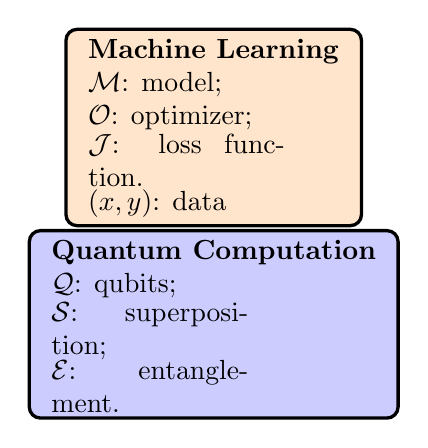
\begin{tikzpicture}[->,>=stealth']

 \node[state, fill=orange!20] (ML) 
 {\begin{tabular}{l}
 \textbf{Machine Learning}\\ 
 \parbox{2.5cm}{$\mathcal{M}$: model;}\\
 \parbox{2.5cm}{$\mathcal{O}$: optimizer;}\\
 \parbox{2.5cm}{$\mathcal{J}$: loss function.}\\
 \parbox{2.5cm}{$(x, y)$: data}
  \end{tabular}
  };
  
  \node[state,
  below of = ML,
  yshift=-1.5cm, fill=blue!20] (QC) 
 {\begin{tabular}{l}
 \textbf{Quantum Computation}\\ 
 \parbox{2.5cm}{$\mathcal{Q}$: qubits;} \\
 \parbox{2.5cm}{$\mathcal{S}$: superposition;}\\
 \parbox{2.5cm}{$\mathcal{E}$: entanglement.}
  \end{tabular}
  };
  
\end{tikzpicture}
\end{frame}


% SLIDE 2 QML
\begin{frame}{Quantum Machine Learning - operating on qubits}

\vspace{1.77cm}

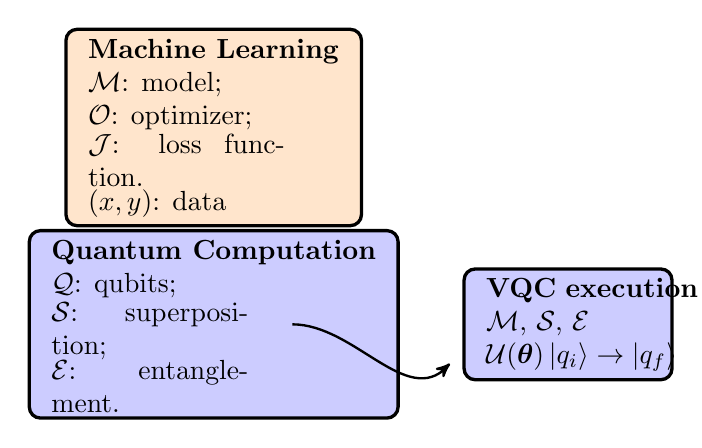
\begin{tikzpicture}[->,>=stealth']

 \node[state, fill=orange!20] (ML) 
 {\begin{tabular}{l}
 \textbf{Machine Learning}\\ 
 \parbox{2.5cm}{$\mathcal{M}$: model;}\\
 \parbox{2.5cm}{$\mathcal{O}$: optimizer;}\\
 \parbox{2.5cm}{$\mathcal{J}$: loss function.}\\
 \parbox{2.5cm}{$(x, y)$: data}
  \end{tabular}
  };
  
  \node[state,
  below of = ML,
  yshift=-1.5cm, fill=blue!20] (QC) 
 {\begin{tabular}{l}
 \textbf{Quantum Computation}\\ 
 \parbox{2.5cm}{$\mathcal{Q}$: qubits;} \\
 \parbox{2.5cm}{$\mathcal{S}$: superposition;}\\
 \parbox{2.5cm}{$\mathcal{E}$: entanglement.}
  \end{tabular}
  };
  
   \node[state,
    right of=QC,
    yshift=0cm,
    anchor=center,
    node distance=4.5cm, 	
    text width=2.5cm, fill=blue!20] (VQC) 
 {%
 \begin{tabular}{l}
  \textbf{VQC execution}\\
  $\mathcal{M}$, $\mathcal{S}$, $\mathcal{E}$ \\
  \parbox{2.8cm}{$\mathcal{U}(\bm{\theta})\ket{q_i} \to \ket{q_f}$}
 \end{tabular}
 };
 
  \draw[line width=0.3mm] (1, -2.5)  to[out=0, in=230] (3, -3);
\end{tikzpicture}

\end{frame}

% SLIDE 3 QML
\begin{frame}{Quantum Machine Learning - natural randomness}

\vspace{1.77cm}

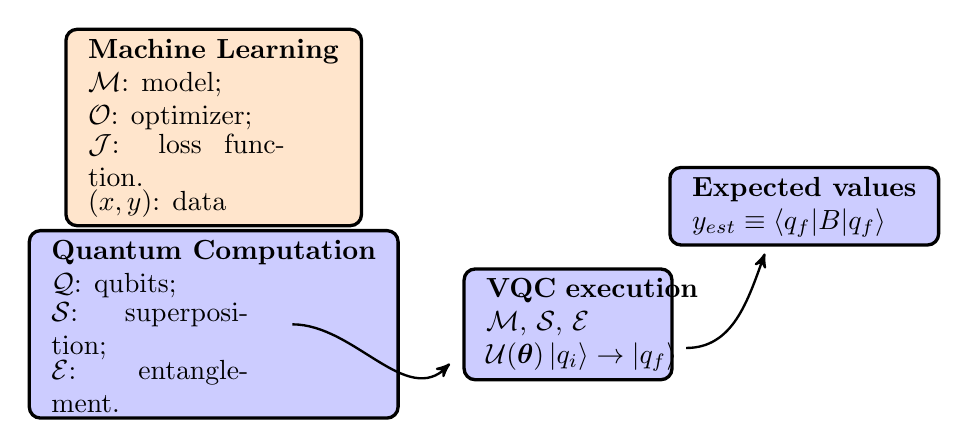
\begin{tikzpicture}[->,>=stealth']

 \node[state, fill=orange!20] (ML) 
 {\begin{tabular}{l}
 \textbf{Machine Learning}\\ 
 \parbox{2.5cm}{$\mathcal{M}$: model;}\\
 \parbox{2.5cm}{$\mathcal{O}$: optimizer;}\\
 \parbox{2.5cm}{$\mathcal{J}$: loss function.}\\
 \parbox{2.5cm}{$(x, y)$: data}
  \end{tabular}
  };
  
  \node[state,
  below of = ML,
  yshift=-1.5cm, fill=blue!20] (QC) 
 {\begin{tabular}{l}
 \textbf{Quantum Computation}\\ 
 \parbox{2.5cm}{$\mathcal{Q}$: qubits;} \\
 \parbox{2.5cm}{$\mathcal{S}$: superposition;}\\
 \parbox{2.5cm}{$\mathcal{E}$: entanglement.}
  \end{tabular}
  };
  
   \node[state,
    right of=QC,
    yshift=0cm,
    anchor=center,
    node distance=4.5cm, 	
    text width=2.5cm, fill=blue!20] (VQC) 
 {%
 \begin{tabular}{l}
  \textbf{VQC execution}\\
  $\mathcal{M}$, $\mathcal{S}$, $\mathcal{E}$ \\
  \parbox{2.8cm}{$\mathcal{U}(\bm{\theta})\ket{q_i} \to \ket{q_f}$}
 \end{tabular}
 };
 
\node[state,
  right of = VQC,
  node distance = 3cm,
  yshift=1.5cm, fill=blue!20] (NSHOT) 
 {\begin{tabular}{l}
 \textbf{Expected values}\\ 
 $y_{est} \equiv \braket{q_f|B|q_f}$
  \end{tabular}
  };
 
  \draw[line width=0.3mm] (1, -2.5)  to[out=0, in=230] (3, -3);
 \draw[line width=0.3mm] (6, -2.8)  to[out=0, in=250] (7, -1.6);
\end{tikzpicture}

\end{frame}


% SLIDE 4 QML

\begin{frame}{Quantum Machine Learning - encoding the problem}

\vspace{1.01cm}
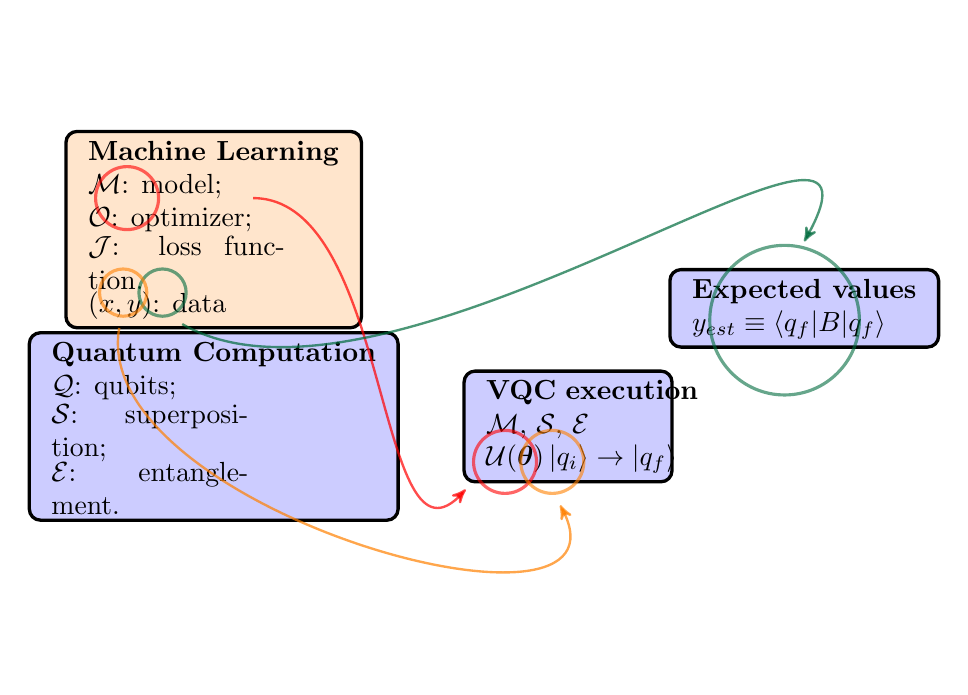
\begin{tikzpicture}[->,>=stealth']

 \node[state, fill=orange!20] (ML) 
 {\begin{tabular}{l}
 \textbf{Machine Learning}\\ 
 \parbox{2.5cm}{$\mathcal{M}$: model;}\\
 \parbox{2.5cm}{$\mathcal{O}$: optimizer;}\\
 \parbox{2.5cm}{$\mathcal{J}$: loss function.}\\
 \parbox{2.5cm}{$(x, y)$: data}
  \end{tabular}
  };
  
  \node[state,
  below of = ML,
  yshift=-1.5cm, fill=blue!20] (QC) 
 {\begin{tabular}{l}
 \textbf{Quantum Computation}\\ 
 \parbox{2.5cm}{$\mathcal{Q}$: qubits;} \\
 \parbox{2.5cm}{$\mathcal{S}$: superposition;}\\
 \parbox{2.5cm}{$\mathcal{E}$: entanglement.}
  \end{tabular}
  };
  
 
 \node[state,
    right of=QC,
    yshift=0cm,
    anchor=center,
    node distance=4.5cm, 	
    text width=2.5cm, fill=blue!20] (VQC) 
 {%
 \begin{tabular}{l}
  \textbf{VQC execution}\\
  $\mathcal{M}$, $\mathcal{S}$, $\mathcal{E}$ \\
  \parbox{2.8cm}{$\mathcal{U}(\bm{\theta})\ket{q_i} \to \ket{q_f}$}
 \end{tabular}
 };
 
\node[state,
  right of = VQC,
  node distance = 3cm,
  yshift=1.5cm, fill=blue!20] (NSHOT) 
 {\begin{tabular}{l}
 \textbf{Expected values}\\ 
 $y_{est} \equiv \braket{q_f|B|q_f}$
  \end{tabular}
  };

  
 \draw[line width=0.3mm, red, opacity = 0.7] (0.5, 0.4)  to[out=0, in=230] (3.2, -3.3);
 \draw[line width=0.3mm, orange, opacity = 0.7] (-1.2, -1.25)  to[out=260, in=300] (4.4, -3.5);
 \draw[line width=0.3mm, cadmiumgreen, opacity = 0.7] (-0.4, -1.2)  to[out=330, in=60] (7.5, -0.15);
  
 
 \draw[red, line width=0.4mm, opacity = 0.6] (3.7,-2.95) circle (0.4 cm);
 \draw[red, line width=0.4mm, opacity = 0.6] (-1.1, 0.4) circle (0.4 cm);
 \draw[cadmiumgreen, line width=0.4mm, opacity = 0.6] (-0.65,-0.8) circle (0.3 cm);
 \draw[cadmiumgreen, line width=0.4mm, opacity = 0.6] (7.25,-1.15) circle (0.95 cm);
 \draw[orange, line width=0.4mm, opacity = 0.6] (4.3,-2.95) circle (0.4 cm);
 \draw[orange, line width=0.4mm, opacity = 0.6] (-1.15,-0.8) circle (0.3 cm);


\end{tikzpicture}
\end{frame}

% SLIDE 5 QML

\begin{frame}{Quantum Machine Learning!}

\vspace{0.25cm}
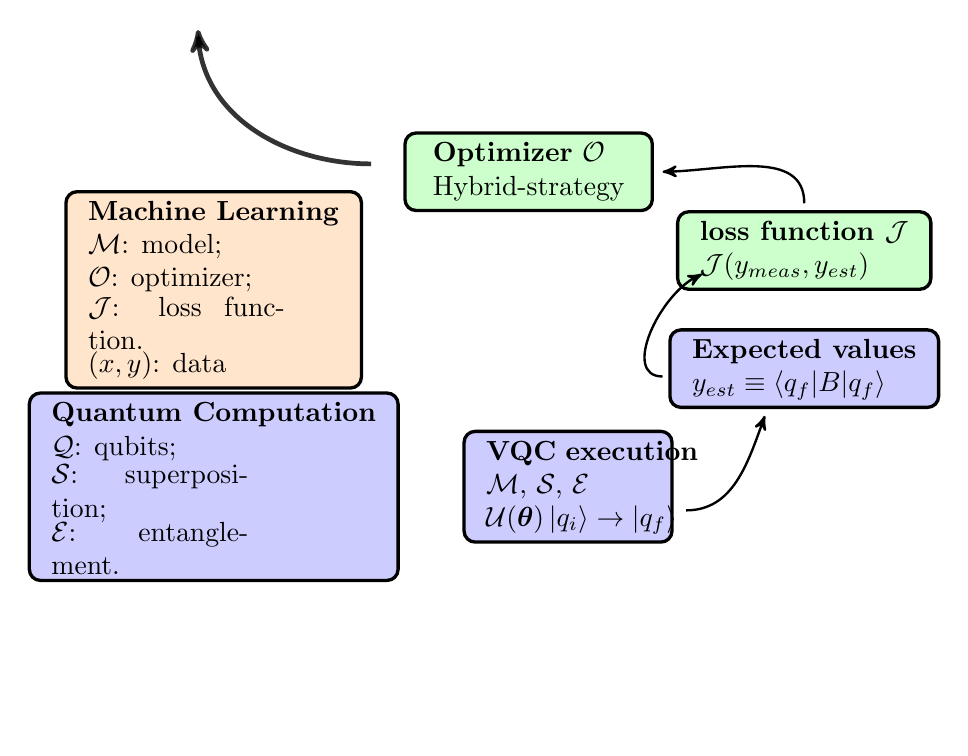
\begin{tikzpicture}[->,>=stealth']


 \node[state, fill=orange!20] (ML) 
 {\begin{tabular}{l}
 \textbf{Machine Learning}\\ 
 \parbox{2.5cm}{$\mathcal{M}$: model;}\\
 \parbox{2.5cm}{$\mathcal{O}$: optimizer;}\\
 \parbox{2.5cm}{$\mathcal{J}$: loss function.}\\
 \parbox{2.5cm}{$(x, y)$: data}
  \end{tabular}
  };
  
  \node[state,
  below of = ML,
  yshift=-1.5cm, fill=blue!20] (QC) 
 {\begin{tabular}{l}
 \textbf{Quantum Computation}\\ 
 \parbox{2.5cm}{$\mathcal{Q}$: qubits;} \\
 \parbox{2.5cm}{$\mathcal{S}$: superposition;}\\
 \parbox{2.5cm}{$\mathcal{E}$: entanglement.}
  \end{tabular}
  };
  

 \node[state,   
  text width=3cm, 
  yshift=1.5cm, 
  right of=ML, 	
  node distance=4cm, 
  anchor=center, fill=green!20] (OPT) 
 {%
 \begin{tabular}{l} 	% content
  \textbf{Optimizer $\mathcal{O}$}\\
  Hybrid-strategy
 \end{tabular}
 };
 
 \node[state,
    right of=QC,
    yshift=0cm,
    anchor=center,
    node distance=4.5cm, 	
    text width=2.5cm, fill=blue!20] (VQC) 
 {%
 \begin{tabular}{l}
  \textbf{VQC execution}\\
  $\mathcal{M}$, $\mathcal{S}$, $\mathcal{E}$ \\
  \parbox{2.8cm}{$\mathcal{U}(\bm{\theta})\ket{q_i} \to \ket{q_f}$}
 \end{tabular}
 };
 
\node[state,
  right of = VQC,
  node distance = 3cm,
  yshift=1.5cm, fill=blue!20] (NSHOT) 
 {\begin{tabular}{l}
 \textbf{Expected values}\\ 
 $y_{est} \equiv \braket{q_f|B|q_f}$
  \end{tabular}
  };
  
  \node[state,
  above of = NSHOT,
  node distance = 1.5cm,
  yshift=0cm, fill=green!20] (J) 
 {\begin{tabular}{l}
 \textbf{loss function $\mathcal{J}$}\\ 
 $\mathcal{J}(y_{meas}, y_{est})$
  \end{tabular}
  };
  

 \draw[line width=0.3mm] (6, -2.8)  to[out=0, in=250] (7, -1.6);
 \draw[line width=0.3mm] (5.7, -1.1)  to[out=180, in=200] (6.2, 0.2);
 \draw[line width=0.3mm] (7.5, 1.1)  to[out=90, in=0] (5.7, 1.5);
 \draw[line width=0.6mm, opacity=0.8] (2, 1.6)  to[out=180, in=270] (-0.2, 3.3);
 
 \draw[line width=0.3mm, orange, opacity = 0.0] (-1.2, -1.25)  to[out=260, in=300] (4.4, -3.5);

\end{tikzpicture}

\end{frame}

\section{References}


\begin{frame}{Let's jump to the console}
\large
\faArrowCircleRight\,\, We leave some references and links thanks to which you can use our codes and read more about the project:

\begin{multicols}{2}
    
\begin{itemize}
\item[\faCode] open-access codes for personal coding or contributing:
    \begin{itemize}[noitemsep]
        \item[\faGithub]  \href{https://github.com/qiboteam/qibo}{the \texttt{qibo} package};
        \item[\faGithub]  \href{https://github.com/qiboteam/qibolab}{the \texttt{qibolab} package};
        \item[\faGithub]  \href{https://github.com/qiboteam/qibocal}{the \texttt{qibocal} package};
    \end{itemize}
 \vspace{1cm}

\item[\faBook] our official \href{https://qibo.science/}{webpage}, with the following documentations:
    \begin{itemize}[noitemsep]
        \item[\faLeanpub]  \href{https://qibo.science/docs/qibo/stable}{the \texttt{qibo} docs};
        \item[\faLeanpub]  \href{https://qibo.science/docs/qibolab/stable}{the \texttt{qibolab} docs};
        \item[\faLeanpub]  \href{https://qibo.science/docs/qibocal/stable}{the \texttt{qibocal} docs};
    \end{itemize}
\end{itemize}
\end{multicols}

\faCloudDownload\,\, the \href{https://colab.research.google.com/drive/1Mxxb2iQzkg-sKQxZiBin3cN9P-LzIa0E\#scrollTo=9hWH63k5610I}{Colab notebook} we are going to run together.

\end{frame}


\end{document}
